\chapter{Estrategias de planificación de queries}
\label{cap:planificacion}
Los motores de búsqueda verticales son sistemas dedicados a un solo propósito e ideado con el propósito de lidiar con cargas de trabajos dinámicas. Un ejemplo de un motor de búsqueda vertical es un motor de publicidad que ejecuta una consulta cada vez que un usuario abre un correo electrónico en por ejemplo, el servicio de \textit{Yahoo! mail}; de esta forma se muestra publicidad de acuerdo al contenido del correo electrónico. Eventualmente millones de usuarios concurrentes están conectados a sus correos electrónicos, por lo que la carga de trabajo esperada para el motor de búsqueda puede llegar a órdenes de las cien mil consultas por segundo \citep{Gil-Costa:2013}. Adicionalmente, el hecho que las actualizaciones en un motor de búsqueda vertical ocurran con mayor frecuencia que en uno de propósito general, hace que el diseño de los algoritmos para procesar las \textit{queries} sea diferente; también se debe permitir la actualización del índice invertido.

Por lo anteriormente mencionado, se hace imperioso tener un sistema diseñado que soporte altas cargas de trabajo, y las respuestas a consultas esten en una cota de tiempo aceptable para el usuario sin mermar la calidad de los resultados obtenidos. También es necesario que las estructuras de datos y los algoritmos implementados soporten la concurrencia entre las transacciones de lecturas y escrituras; dicho de otra forma, eventualmente el motor de búsqueda tendrá que dejar de procesar consultas para poder servir las transacciones de escritura que actualizan el índice invertido.

A continuación se muestra las diferentes estrategias de planificación de transacciones de lectura abordadas en el presente trabajo utilizando diferentes enfoques; se presentan tres enfoques diferentes: El primero consiste en crear bloques de consultas en donde previamente a cada una de ellas se le asigna el número de hebras que utilizará en su resolución, luego el bloque es procesado en paralelo por los diferentes hilos de ejecución asignados; El segundo enfoque corresponde a unidades de trabajos, en la que a cada \textit{query} se le asigna un número determinado de unidades de trabajo y los \textit{threads} compiten por ellas desde una cola; (3) El tercer enfoque y último es el más básico, cada hilo de ejecución se hace cargo de una consulta y lleva a cabo su procesamiento, en este enfoque la competencia entre los hilos de ejecución es por las consultas. 


\section{Estrategias por bloques}
\label{scheduling:bloques}
Un sistema de planificación de un motor de búsqueda trabaja en un contexto \textit{online}, esto significa que desconoce las transacciones que vendrán en el futuro y que cuando llega una nueva transacción de lectura, se debe tomar una decisión rápida acerca de qué hacer con ella. Adicionalmente, una transacción de lectura debe ser resuelta dentro de una cota superior de tiempo, al cual llamaremos $t_limite$. En el contexto del presente trabajo, para que el planificador tome una decisión con respecto a una query, debe conocer de ella (1) su tiempo de ejecución y (2) el número de hebras con los que será resuelta. El tiempo de ejecución de cada consulta se obtiene utilizando los métodos de predicción de tiempos mostrados en el Capítulo \ref{cap:prediccion}; una vez que se predice el tiempo esperado $t_esperado$ de cada query para 1,2,4,8 y 16 threads, se asigna el numero de hilos de ejecución tal que se cumpla que $t_esperado < t_limite$, de esta forma se satisface la condición de que todas las consultas deben ser resueltas en una cota superior de tiempo previamente definida.

\begin{figure}[!th]
\centering
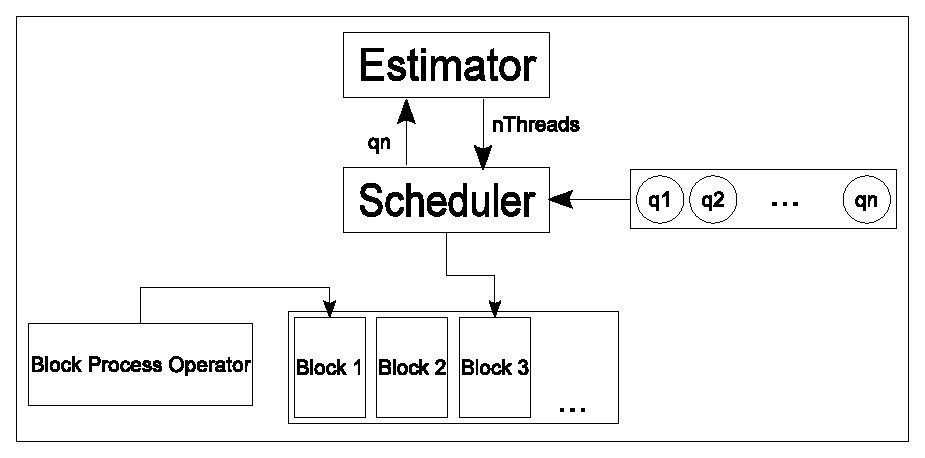
\includegraphics[scale=.75]{images/scheduler_bloques.eps}
\caption{Enfoque de planificación para estrategias por bloques}
\label{fig:schedulerbloques}
\end{figure}  

Bajo el contexto de un motor de búsqueda en el que se debe planificar transacciones de lecturas que eventualmente serán resueltas de forma paralela por diferentes hilos de ejecución, existe una estrategia teórica llamada FR que aborda este problema \citep{Ye:2007} y se adapta a nuestro escenario de un motor de búsqueda vertical; esta estrategia del estado del arte da pie para que en el presente trabajo de tesis se proponga dos nuevas estrategias siguiendo el mismo enfoque de FR, pero estas enfocadas principalmente en mejorar la asignación de consultas a bloques, para así reducir el tiempo ocioso de las hebras. 
En la Figura \ref{fig:schedulerbloques} se muestra el proceso completo del presente enfoque; las consultas que llegan al sistema las recibe el planificador \textit{scheduler} y las envía al estimador (\textit{estimator}), que calcula el número adecuado de hilos de ejecución para la consulta tal que la consulta sea resuelta en un tiempo inferior al tiempo límite $t_limite$. Una vez que a la \textit{query} se le predice el tiempo de ejecución y el número de \textit{threads} a utilizar, este planifica la consulta en algún bloque correspondiente depenediendo de la política que se este utilizando. A continuación se muestran las diferentes estrategias propuestas. 

\subsection{Estrategia FR}
\label{scheduling:fr}
La estrategia FR posee como requisito que cada una de las consultas a planificar se le haya asignado el número de hebras con las cuales se resolverá; esto se hará siguiendo el esquema \ref{fig:schedulerbloques}. Como se dijo anteriormente, a cada consulta se asignará la cantidad mínima de hebras tal que el tiempo en resolver la consulta sea menor al tiempo límite $t_limite$.

Por lo explicado en el párrafo anterior, el algoritmo FR asume que cada \textit{query} que llega al motor de búsqueda posee el número de hebras que debe utilizarse en su resolución. Utilizando esta información, la estrategia hace una clasificación de cada consulta entre \textit{Big} y \textit{Small}, con el objetivo de crear estructuras de datos denominadas \textit{Rooms} y {Walls}, en donde cada \textit{Wall} y cada {Room} estará formado solo por consultas de tipo \textit{Big} y \textit{Small} respectivamente. Ambas estructuras de dato tienen un número máximo de máquinas disponibles para procesar las transacciones de lectura. Una \textit{query} es \textit{Big} si el número de máquinas requeridas para procesarla es $m$ (siendo m el número de máquinas disponibles en el sistema), de lo contrario la \textit{query} es \textit{Small}. La idea del algoritmo es crear bloques de consultas (\textit{Wall} y \textit{Room}), que serán procesadas en paralelo por el proceso que resuelve las consultas. 

% Debe ir una imagen explicando cómo se irán formando los bloques

% ----  Descripción del algoritmo ----
Como se puede ver en el Algoritmo \ref{alg:fr}, cuando una nueva \textit{query} llega al sistema, esta se analiza si es de tipo \textit{Big} o \textit{Small}; esto se hace en el método \textit{isBig()}, que retorna verdadero si es que el número de máquinas requeridas para procesar la consulta es igual al máximo de máquinas disponibles en el sistema, de lo contrario retorna falso y la transacción es clasificada como \textit{Small}. Si la consulta es \textit{Big}, entonces se crea una estructura de dato \textit{Wall}, se planifica la \textit{query} en el bloque y esta se inserta en la lista de planificación \textit{SchedulingList} que contendrá todos los bloques con las consultas ya planificadas. Si se está en presencia de una transacción de lectura de tipo \textit{Small}, se busca algún bloque de tipo \textit{Room} para planificarla; para planificar esta consulta, el bloque debe satisfacer dos condiciones: (1) No debe estar completo, es decir, debe tener threads disponibles, y (2) No debe haber sido procesado aún. Finalmente, si eventualmente no se encuentra algún bloque disponible para planificar la \textit{query}, entonces se crea un nuevo bloque \textit{Room}, se planifica la consulta al bloque y este bloque es insertado en lista de \textit{scheduling}. Cabe destacar que se dice que un bloque está abierto (\textit{isOpen()}) cuando las consultas presentes en el bloque no han ocupado todos los hilos de ejecución disponibles o cuando el proceso de ejecución ya ha procesado el bloque. Es importante también notar que las estructuras de datos de tipo \textit{Wall} estarán formadas solo por una transacción de lectura de tamaño máximo.
%----- Fin descripción algoritmo ----

\begin{algorithm}[!th]
\caption{\em $schedulerFR::assignQuery(L, Q)$: Planificación de consulta estrategia FR}
\label{alg:fr}
\begin{algorithmic}[1]
\REQUIRE Una SchedulingList $L$ en donde se hará la planificación, QueryObject $Q$ a planificar
\ENSURE SchedulingList $L$ con la nueva query planificada

\IF {$isBig(query)$}
	\STATE $block = new Wall();$
	\STATE $block \rightarrow addQuery(query);$
	\STATE $L \rightarrow addBlock(block);$
\ELSE
	\STATE $asignada = false;$
	\FOR {$ i = L \rightarrow firstOpenBlockLocked() ... L \rightarrow size()$}
		\STATE $room\_block = L \rightarrow getBlockLocked(i);$
		
		\IF {$(room\_block \rightarrow isOpen()) AND 
				(room\_block \rightarrow freeThreads() >= query \rightarrow getThreads())$
			}
			\STATE $room\_block \rightarrow addQuery(query)$
			\STATE $asignada = true$
			\STATE $break;$
		\ENDIF
	\ENDFOR
	
	\IF {$!(asignada)$}
		\STATE $block = new Room();$
		\STATE $block \rightarrow addQuery(query);$
		\STATE $L \rightarrow addBlockLocked(block);$		
	\ENDIF
\ENDIF

\end{algorithmic}
\end{algorithm}


% --- Descripción proceso ---
En la Figura X se presenta un ejemplo de ejecucion la estrategia FR. Ya han llegado al sistema consultas: q0 (2 threads), q1 (16 threads), q2 (4 threads), q3 (2 threads), q4 (2 threads), q5 (8 threads) y q6 (16 threads). Se puede ver cómo se van formando las estructuras de datos llamadas \textit{Rooms} y \textit{Walls}. Suponer que eventualmente arriba al sistema una nueva consulta que será resuelta con 8 \textit{threads}, entonces el algoritmo verifica en primera instancia la $Room_0$, sin embargo, en esta estructura no hay suficientes \textit{threads} disponibles para procesar la consulta (posee solo 6 disponibles). Finalmente la planifica en la $Room_1$.

\begin{figure}[!th]
\centering
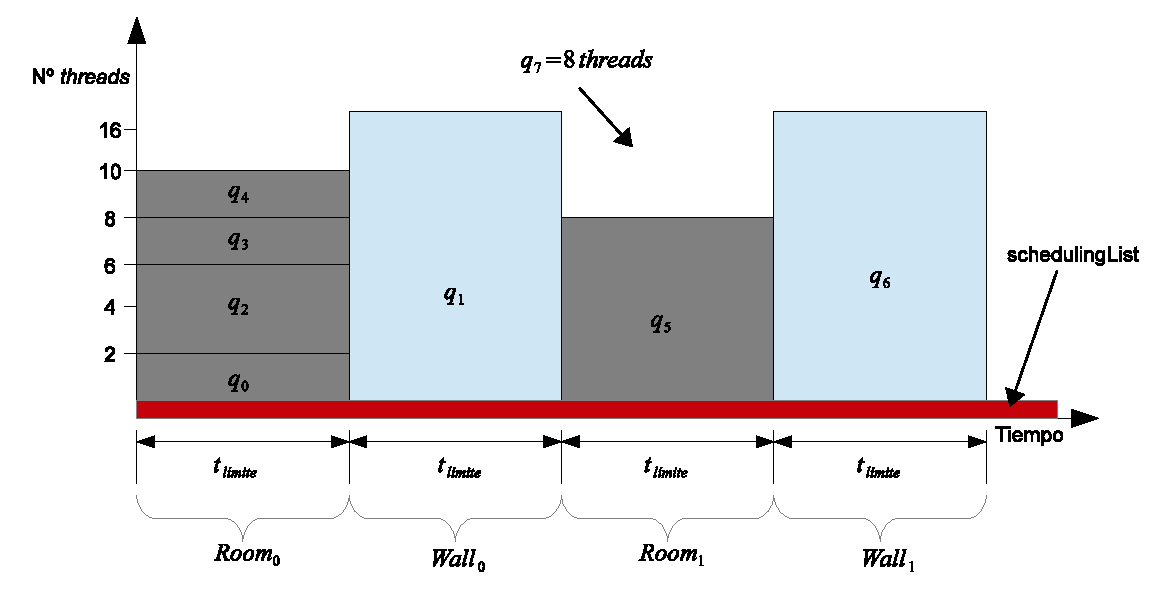
\includegraphics[scale=.75]{images/proceso_FR.eps}
\caption{Ejemplo de procesamiento de la estrategia FR}
\label{fig:proceso_FR}
\end{figure} 
%----- Fin descripción proceso ----

\subsection{Estrategia Times}
\label{scheduling:times}
Se intuye que una de las desventajas de la estrategia FR es que al planificar una consulta en algún bloque, solo verifica si es que este posee el número de threads desocupados suficientes tal que sea mayor o igual al número de threads requerido por la consulta. Esto puede generar pérdida de eficiencia importante en los procesamientos de los bloques, puesto que algunas transacciones de lecturas pueden tomar mayor tiempo en ser procesadas y los hilos de ejecución que ya han terminado su trabajo estarán ociosos esperando por otros para continuar con el siguiente bloque. Para abordar esta posible pérdida de eficiencia, se diseña una política de planificación alternativa en donde además de tomar en cuenta el número de threads disponible en cada bloque (como en la estrategia anterior), se toma en cuenta el tiempo esperado de la transacción de lectura.

Cada consulta $q$ tiene asociado un número de threads $NT_q$ y un tiempo $t_predicho$, que es el tiempo en que se espera que la consulta sea resuelta con $NT_q$ hilos de ejecución. La idea de esta estrategia es separar las transacciones de lectura que tengan tiempos de procesamiento muy diferentes en bloques distintos, es decir, se crearán bloques con consultas que tengan poca diferencia de tiempo unas de otra, de esta forma se quiere reducir el tiempo que se podría perder entre un bloque y otro por el desbalance de carga de los \textit{threads}. Cada bloque $B$ tendrá un tiempo $t_B$, que será el tiempo de la consulta con menor tiempo dentro del bloque. La métrica establecida para que una transacción de lectura que llega al sistema sea planificada en un bloque, es que el tiempo del bloque $t_B$ no sea el doble del tiempo de la consulta $t_q$ entrante, y viceversa. Si esta condición falla, entonces significa que la consulta $q$ que se está intentando planificar posee tiempos que se escapa a los rangos de tiempo del bloque $B$. A continuación se muestra el algoritmo para la presente estrategia

\begin{algorithm}[!th]
\caption{\em $schedulerTimes::assignQuery(L, Q)$: Planificación de consulta estrategias Times}
\label{alg:times}
\begin{algorithmic}[1]
\REQUIRE Una SchedulingList $L$ en donde se hará la planificación, QueryObject $Q$ a planificar
\ENSURE SchedulingList $L$ con la nueva query planificada
	\STATE $blocks_viewed = 0$
	
	\FOR {$ i = L \rightarrow firstOpenBlockLocked()...L \rightarrow sizeLocked()$}
		\STATE $block = lista\_bloques \rightarrow getBlockLocked(i);$
		
		\IF {$block \rightarrow isOpen() AND block \rightarrow freeThreads() \geq query \rightarrow getThreads()$}
			\STATE $queries = block \rightarrow getQueries();$
			\STATE $tiempo\_min = queries[0] \rightarrow getEstimatedTime();$
			
			\FOR {$ j = 1 ...queries->size()$}
				\IF {$queries[j] \rightarrow getEstimatedTime() < tiempo_min$}
					\STATE $tiempo\_min = queries[j] \rightarrow getEstimatedTime();$
				\ENDIF
			\ENDFOR
			
			\IF {$tiempo\_min < estimated\_time$}
				\STATE $diff = 2*tiempo_min - estimated_time;$
			\ELSE
				\STATE $diff = 2*estimated_time - tiempo_min;$
			\ENDIF
			
			\IF {$diff < 0$}
				\STATE $diff = 0.0-diff;$
				\IF {$diff < best_diff$}
					\STATE $best_diff = diff;$
					\STATE $best_block = i;$
				\ENDIF
			\ELSE
				\STATE $valido = true;$
			\ENDIF
			
			\IF {$ valido $}
				\STATE $block \rightarrow addQuery(query);$
				\STATE $asignada = true;$
				\STATE $break;$
			\ENDIF
			
			\STATE $bloques_revisados++;$
			
			\IF {$bloques_revisados \geq max_bloques_rev$}
				\STATE $break;$
			\ENDIF
			
		\ENDIF
		
	\ENDFOR
	
	\IF {$ ! asignada $}
		\IF {$ (bloques\_revisados \geq max\_bloques_rev) $}
			\STATE $block = lista\_bloques \rightarrow getBlockLocked(best\_block);$
			\STATE $block \rightarrow addQuery(query);$
		\ELSE
			\STATE $block = new QueryBlock();$
			\STATE $block \rightarrow addQuery(query);$
			\STATE $lista\_bloques \rightarrow addBlockLocked(block);$
			
		\ENDIF	
	\ENDIF

\end{algorithmic}
\end{algorithm}




\subsection{Estrategia TimesRanges}
\label{scheduling:fr}


\section{Estrategia unidades de trabajo}
\label{scheduling:unidadestrabajo}
Decir que aquí para planificar se necesita conocer las unidades de trabajos requeridas en vez de threads como en las estrategias por bloques.

Con respecto a los esquemas explicados hasta ahora, el esquema 1TQ tiene la ventaja que no solo requiere menos control, sino que también permite a los hilos de ejecución trabajar sin pausa mientras un \textit{batch} de consultas está siendo procesado. En esta sección se propone un esquema híbrido basado en unidades de procesamiento (\textit{Processing Units}) que aproveche las ventajas de ambos enfoques. (se requiere ver el tema de bloques).
En este nuevo esquema de planificación, las consultas pasan a través de una fase en la cual cada \textit{query} es evaluada y se determina un apropiado número de unidades de procesamiento (\textit{processing units}) para poder resolver dicha consulta. Este proceso es llevado a cabo de manera similar al proceso en donde se determina la cantidad de \textit{threads} apropiados para resolver una determina transacción de lectura. Este número de unidades de procesamiento es creado y asociado a cada consulta, finalmente se guarda en una cola de unidades de trabajo. Un conjunto de \textit{threads} consumidores extraen las unidades desde la cola y las procesa independientemente. Cuando un \textit{thread} finalice el procesamiento de la unidad de trabajo actual automáticamente leerá la siguiente unidad de trabajo desde la cola. 
Generalmente lo que se hace habitualmente es estimar el número de \textit{threads} con el que se resolverá la consulta, como se muestra en la Figura \ref{fig:unit_process} en este nuevo enfoque se intenta estimar el número de unidades de trabajo con el que se resolverá cada consulta. Además, se debe controlar el acceso concurrente de los hilos de ejecución a la cola de unidades de trabajo, de tal manera que solo un thread tenga acceso exclusivo a la estructura de datos. 

\begin{figure}[!th]
\centering
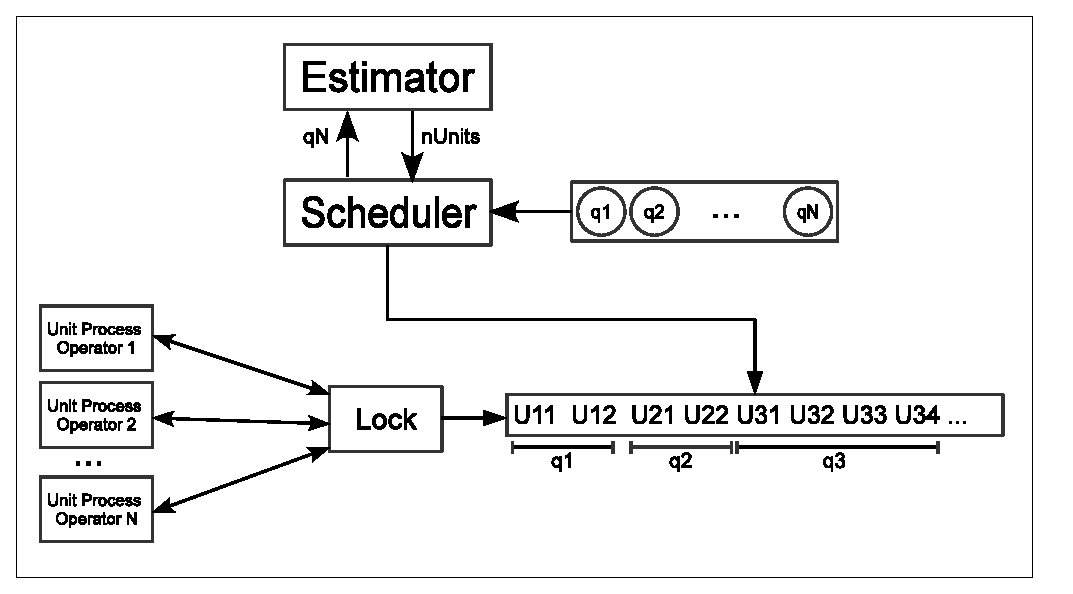
\includegraphics[scale=.75]{images/unit_process.eps}
\caption{Procesamiento de consultas utilizando unidades de trabajo}
\label{fig:unit_process}
\end{figure}

El procesamiento de cada hilo de ejecución es una versión de Wand con heap compartido (SH), adaptado de manera tal que cada unidad de trabajo es resuelta independientemente de si existen otras unidades siendo procesada al mismo tiempo o no. La única excepción es que la unidad que inicializa la consulta es siempre ejecutada antes del resto de las otras unidades de la misma consulta y la entrega de resultados se hace una vez que todas las unidades de trabajo de la \textit{query} han finalizado. Este enfoque híbrido permite reducir el tiempo perdido al final de cada \textit{batch} sin generar una importante pérdida de trabajo mientras las \textit{queries} del \textit{batch} están siendo procesadas.



\section{Estrategia \textit{1TQ}}
\label{scheduling:baseline}
Un simple camino para construir un sistema que responda a múltiples consultas simultáneamente usando múltiple hilos de ejecución, es usando estos hilos de manera independiente. Para hacer esto se debe mantener un conjunto de \textit{threads} consumidores que trabajarán en paralelo y se encargarán de resolver las \textit{queries} secuencialmente (una a una) desde una misma cola, esto es lo que en este trabajo se denomina estrategia de Un Thread Por Query (1TQ). En la Figura \ref{fig:1TQ} se puede apreciar el esquema de ejecución en donde cada uno de los procesos genera una petición de alguna consulta en la cola, si quedan \textit{queries} por procesar entonces se le asigna al proceso una consulta que tendrá que resolver de manera secuencial. Se debe tener en cuenta que cada vez que un proceso genera una solicitud de \textit{query}, se bloquea la estructura de datos que contiene las consultas a procesar y luego se procesa la solicitud, de esta forma se asegura un acceso seguro por parte de los distintos \textit{threads}. 

\begin{figure}[H]
\centering
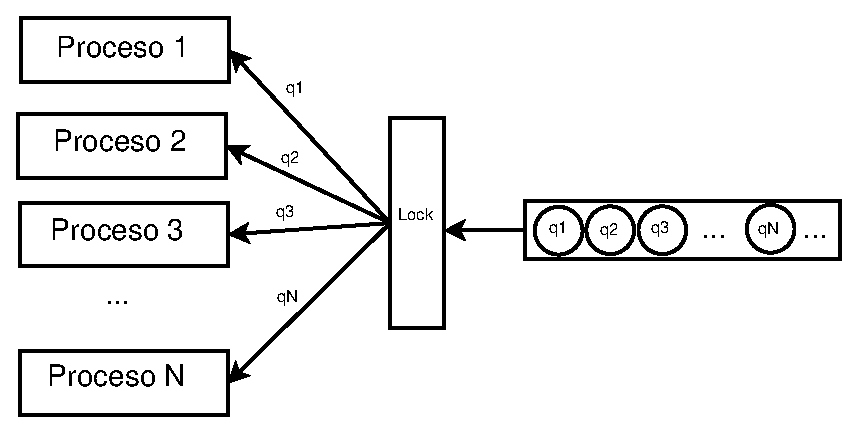
\includegraphics[scale=.75]{images/1TQ.eps}
\caption{Ejemplo de procesamiento estrategia 1TQ}
\label{fig:1TQ}
\end{figure}

Este esquema tiene la ventaja que es simple y fácil de implementar y controlar. Sin embargo, existen sistemas de recuperación de la información como los motores de búsqueda verticales que cuando están ejecutando \textit{batches} de \textit{queries} deben parar su ejecución porque transacciones de escritura han llegado al sistema, y este deben actualizar la información del índice invertido. Solo después de la fase de actualización el sistema es capaz de ejecutar el siguiente \textit{batch} de transacciones de lectura. Al final de cada conjunto de consultas, es posible que algunos hilos de ejecución del sistema finalicen su trabajo y que no tengan más \textit{queries} para procesar, por lo que ellos tienen que esperar que los \textit{threads} restantes finalicen su trabajo antes que el sistema entre en la fase de actualización de su índice invertido o bien, se pase a la ejecución del siguiente \textit{batch} de consultas.
Sin embargo, aunque cada hilo de ejecución está secuencialmente ejecutando una transacción de lectura diferente, algunas de estas operaciones puede tomar un tiempo cosiderable, de esta forma se produce una importante pérdida de eficiencia, aunque la intuición nos dice que esto se puede mitigar con \textit{queries} que requieran poca cantidad de tiempo para ser procesada (trabajos pequeños o \textit{small jobs}). 
En la Figura \ref{fig:small_jobs} queda reflejado lo dicho en el párrafo anterior. Si los trabajos que cada \textit{thread} está ejecutando son pequeños, entonces probablemente la pérdida de trabajo al final de cada \textit{batch} de consultas será menor al trabajo que se pierde cuando los trabajos son grandes (ver Figura \ref{fig:large_jobs}).  


\begin{figure}[H]
\centering
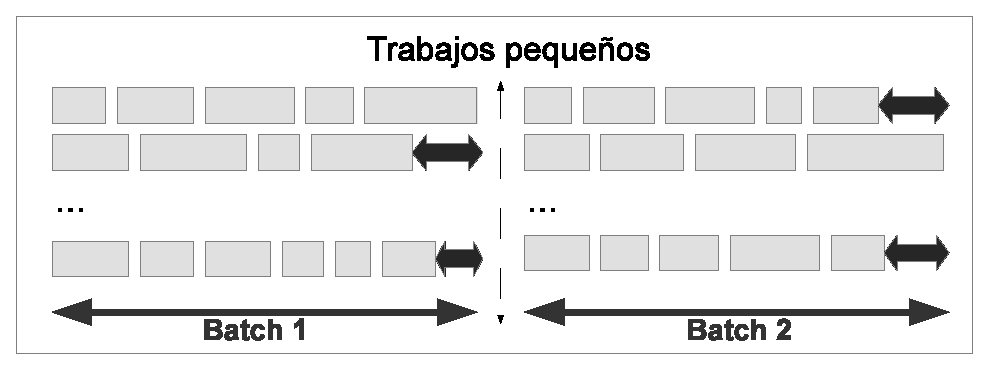
\includegraphics[scale=.75]{images/small_jobs.eps}
\caption{Ejecución en paralelo de \textit{small jobs}}
\label{fig:small_jobs}
\end{figure}

\begin{figure}[H]
\centering
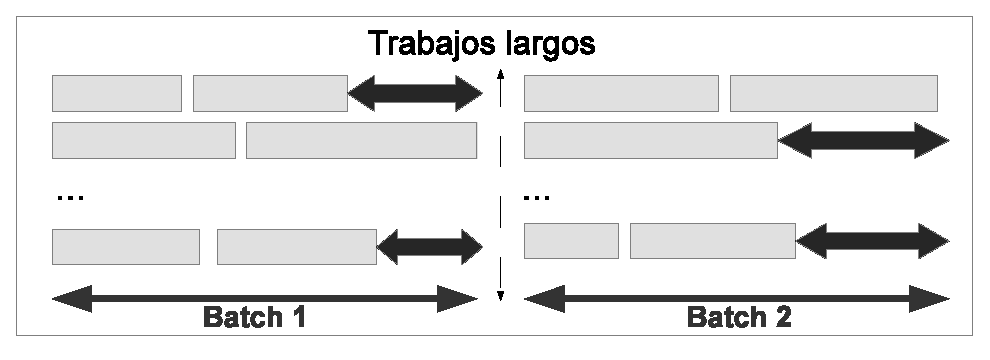
\includegraphics[scale=.75]{images/large_jobs.eps}
\caption{Ejecución en paralelo de \textit{large jobs}}
\label{fig:large_jobs}
\end{figure}